\chapter{Parameter Analyse}

Ein wesentliches Ziel dieser Arbeit ist es das Delf-Verfahren insbesondere für den Anwendungsfall des Retrievals von historischen Abbildungen zu optimieren. Hierfür werden ein Reihen an Parametern entlang der Delf-Pipeline variiert und ihre Einflüsse, auf die Retrievalergebnisse analysiert.
Die benötigte Rechenleistung zur Durchführung der Experimente wird freundlicherweise vom 
Zentrum für Informationsdienste und Hochleistungsrechnen (ZIH) an der TU Dresden zur Verfügung gestellt. Das verwendete HPC-DA System\footnote{\url{https://tu-dresden.de/zih/hochleistungsrechnen/hpc}, zuletzt besucht am 28.07.20} ermöglicht es viele Experimente parallel und effizient durchzuführen, sodass auch im zeitlich überschaubaren Rahmen dieser Arbeit eine große Anzahl unterschiedlicher Konfigurationen getestet werden können.

\section{Hyperparameteroptimierung der Trainingsphasen}
Die ersten Experimentalreihen befassen sich mit den Trainingsphasen des Delf-Verfahrens. Um bei späteren Retrievalversuchen gute Ergebnisse erzielen zu können, benötigt man Modelle die in der Lage sind aussagekräftige Bildrepräsentationen zu erstellen. Für die Experimente zum Modelltraining wird dabei angenommen, dass die Güte, der von einem Modell erzeugten Deskriptoren bzw. der von einem Modell getroffenen Auswahl an Deskriptoren positiv mit der Fähigkeit, der Modelle korreliert die beim Training gestellte Klassifikationsaufgaben zu lösen. Um die Modelle zu bewerten wird daher der Fehler, in Form der Kreuzentropie betrachtet, der auftritt wenn das Modell einen Validierungsdatensatz klassifiziert. Vor Beginn jedes Experiments werden zufällig $20\%$ der Trainingsbilder (siehe Kap. \ref{trainingsdata} auf Seite \pageref{trainingsdata}) für die Validierung ausgewählt. Die Validierungsdaten stehen dem Modell während des Trainingsprozesses nicht zur Verfügung. Daher können sie genutzt werden, um zu überprüfen, ob ein Modell auch auf ungesehenen Daten vergleichbare Ergebnisse erzielt.
\\
Der Erfolg des Trainingsprozesses hängt wesentlich von der zu trainierenden Architektur und der vorhandenen Datenlage ab. Einfluss haben außerdem Parameter, die den Ablauf des Trainingsprozesses beeinflussen. Die Experiments, die in diesem Abschnitt besprochen werden befassen sich mit der Suche nach optimalen Werten für drei dieser sogenannten Hyperparameter. Betrachtet wird die Anzahl der Trainingsepochen, die Lernrate, die bestimmt wie stark Netzwerkparameter in einem Optimierungsschritt angepasst werden, sowie der Faktor $\gamma$ mit dem die Lernrate alle $10$ Epochen multipliziert wird\footnote{Als weiterer Hyperparameter wurde weight decay untersucht, allerdings lies sich hier kein signifikanter Einfluss auf den Validierungsfehler feststellen. Die Ergebnisse hierzu finden sich im Anhang ab Seite \pageref{weight_decay}}. Die übrigen Hyperparameter sind für alle Experimente fest gesetzt. Die Modelle werden mit einer Batchgröße von $8$ trainiert und mittels Stochastic Gradient Decent (kurz SGD \footnote{\url{https://pytorch.org/docs/stable/optim.html\#torch.optim.SGD}, zuletzt besucht am 30.07.20}) optimiert. Für die zu untersuchenden Hyperparameter werden jeweils Wertebereiche definiert. Die Länge des Trainings kann zwischen $10$ und $40$ Epochen dauern. Die initiale Lernrate wird zwischen $0.01$ und $0.001$ gewählt und der $\gamma$-Faktor liegt im Bereich zwischen $1$ und $0.1$.
\\
Um den Suchraum effizient erkunden zu können wird das von Norman Koch entwickelte Nnopt-Tool verwendet, um neue Hyperparameterkonfigurationen zu erstellen und auf dem HPC-System zu testen. Das Nnopt-Tool, das auf dem Hyperopt-Paket \cite{hyperopt} von Bergstra, Yamins und Cox basiert, wählt automatisch Werte für die zu untersuchenden Hyperparameter innerhalb der definierten Wertebereiche aus und startet mit diesen Experimente auf dem Großrechner. Ist ein Experiment abgeschlossen erhält Nnopt zur Bewertung der Konfiguration den erzielten Validierungsfehler. Neue Konfigurationen werden bevorzugt in der Nähe von bereits getesteten Konfigurationen erstellt, die gute Ergebnisse erzielt haben. Dies erlaubt es schneller optimale Hyperparameterwerte zu finden, als mit einer zufälliger Suche.
\\
Für das Finetuning wurden auf diese Art $22$ unterschiedliche Konfigurationen getestet. Zunächst lässt sich beobachten, dass fast alle getesteten Konfigurationen Modell erzeugen, die in der Lage sind die Trainingsaufgabe sehr gut zu lösen. Im Schnitt erzielen die trainierten Modelle eine Klassifikationgenauigkeit von $95.13\%$ auf den Validierungsdaten\footnote{Obwohl zum Vergleich der Konfigurationen der Validierungsfehler berechnet wurde, wird die Modellperformanz im Folgenden über die Validierungsgenauigkeit dargestellt, da diese Metrik einfacher zu Verstehen ist.}, wobei $20$ der $22$ Modelle eine Genauigkeit von über $90\%$ erreichen(vgl. Abb.\ref{finetuning_int_end}b). Da auf Grund der guten Ergebnisse nur wenig Potential für Verbesserung besteht und die beobachtet Varianz der Ergebnisse unterschiedlicher Konfigurationen gering ist, werden keine Weiteren Testläufe zur Hyperparameteroptimierung durchgeführt. Es sei jedoch erwähnt, dass sich auf Grund der im Verhältnis zu Größe der Suchraumes geringen Anzahl an Testläufen keine eindeutigen Abhängigkeiten zwischen Hyperparametern und Klassifikationsperformanz ableiten lassen.
\\
Gut beobachten lässt sich der positive Effekt der Nutzung eines vortrainierten Modells zu Initialisierung der Netzwerkparameter. So erreichen alle getesteten Konfigurationen bereits nach der ersten Trainingsepoche eine Validierungsgenauigkeit von über $85\%$ (vgl. Abb.\ref{finetuning_int_end}a). Die initialisierten Parameter müssen nur noch geringfügig angepasst werden, um die neue Trainingsaufgabe zu lösen, weshalb die Modelle schnell große Fortschritte erzielen. 
\\
\begin{figure}[h]
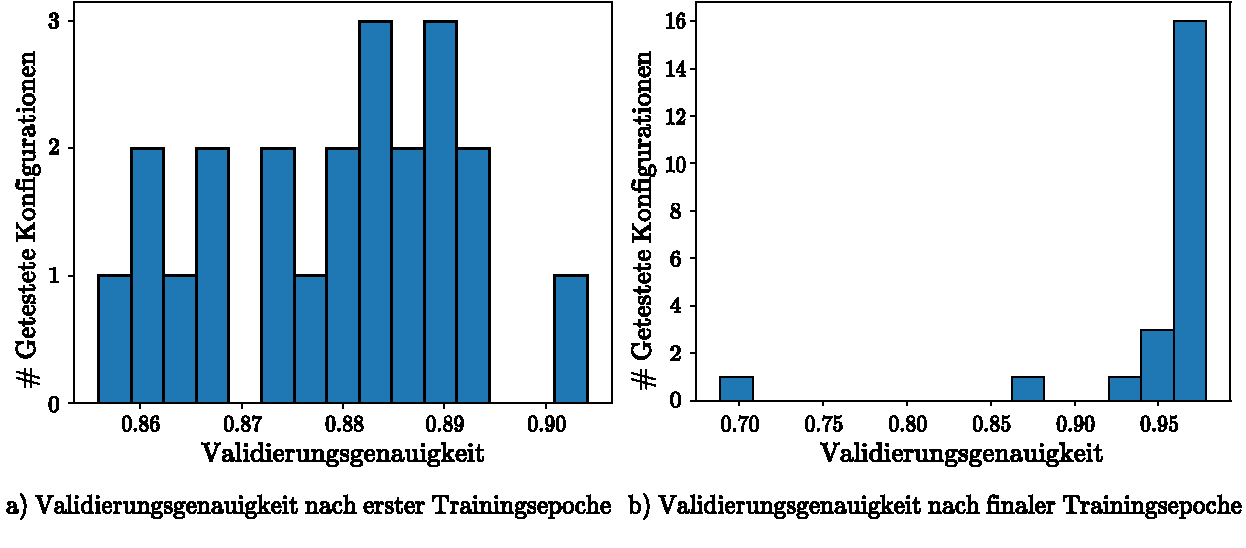
\includegraphics[scale=0.750]{NNOPT/init_and_end_perf_finetuning.pdf}
\caption{Erreichte Klassifikationsgenaugikeit nach der ersten bzw. letzten Epoche des Finetunings, der getesteten Konfigurationen}
\label{finetuning_int_end}
\end{figure}
\\
Betrachtet man die Ergebnisse der Testläufe in Kombination mit den dazugehörigen Hyperparametern (siehe Abb.\ref{finetuning_all}), so scheint die Anzahl an Trainingsepochen keinen signifikanten Einfluss auf die erzielte Validierungsgenauigkeit zu haben. Dies deckt sich mit der Annahme, dass sich Netzwerkparameter mittles Finetuning in wenigen Epochen optimieren lassen. Betrachtet man den Trainingsverlauf des Finetunings (vgl. Abb. \ref{finetuning_lr_gamma_verlauf}), so stellt man fest, das für die meisten Konfigurationen nach $10-15$ Epochen keine großen Verbesserungen mehr im Hinblick auf die Validierungsgenauigkeit erzielt werden.  
\begin{figure}[h]
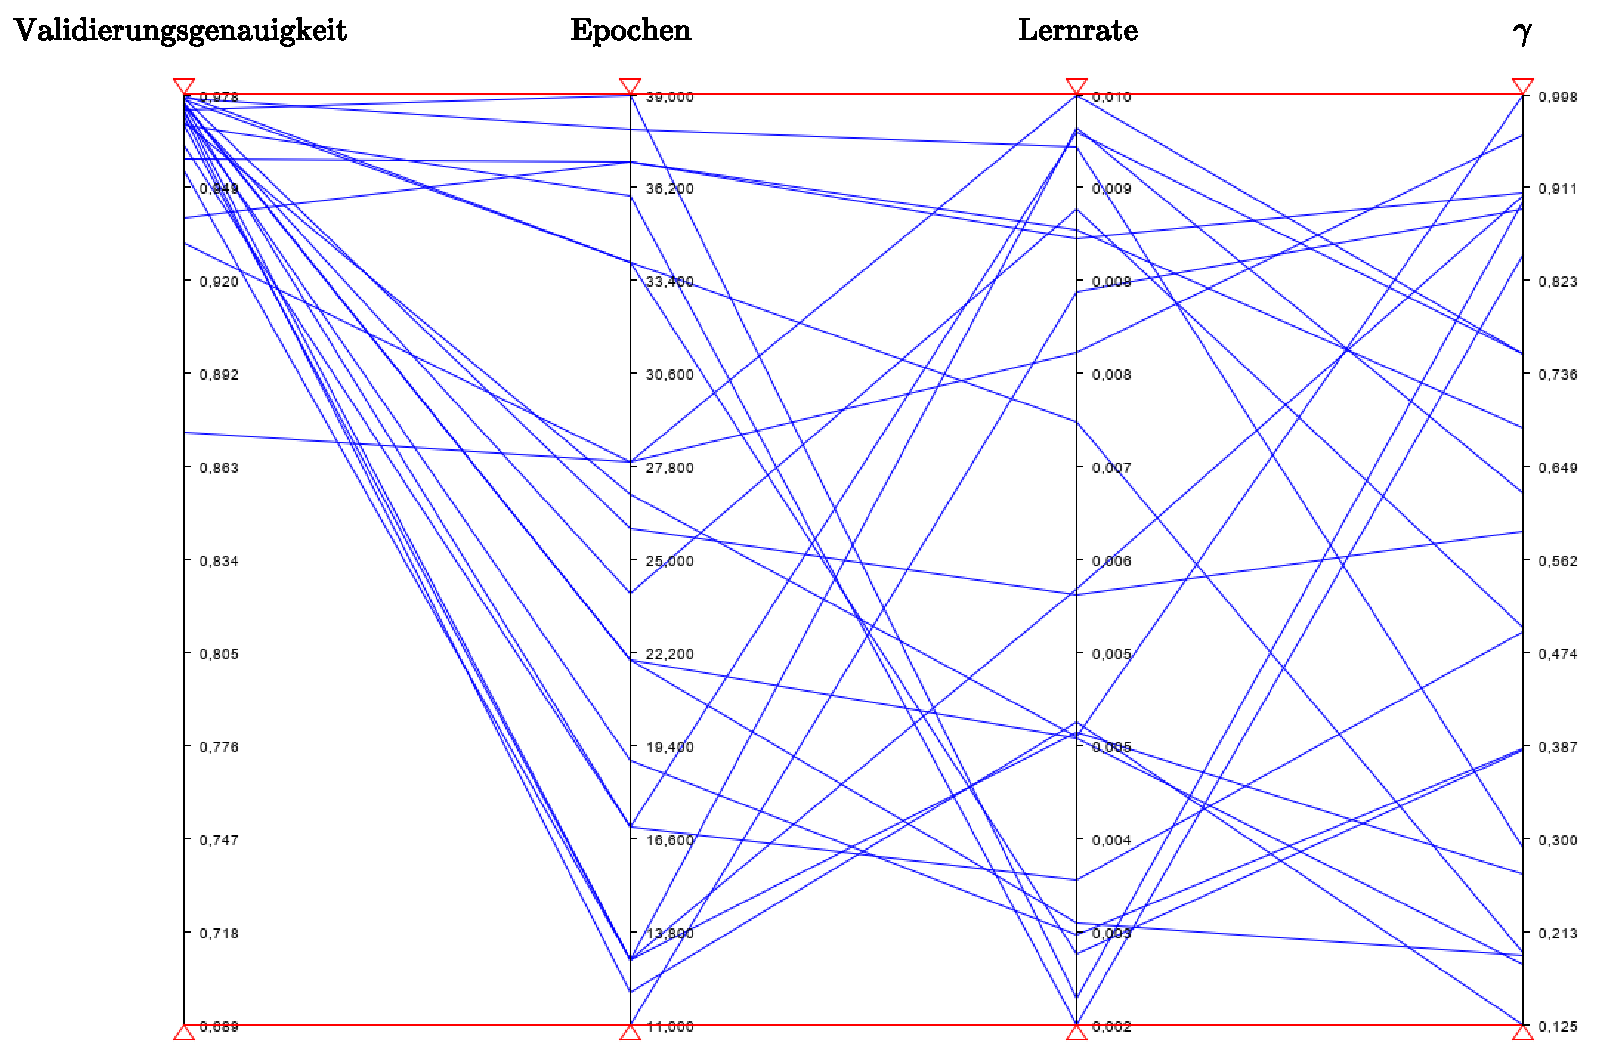
\includegraphics[scale=0.6]{NNOPT/finetuning_all.pdf}
\caption{Parallele Darstellung der getesteten Konfigurationen des Finetunings. Jede Linie repräsentiert einen Konfiguration und die von ihr erzielte Validierungsgenauigkeit.}
\label{finetuning_all}
\end{figure}
\\
\begin{figure}[h]
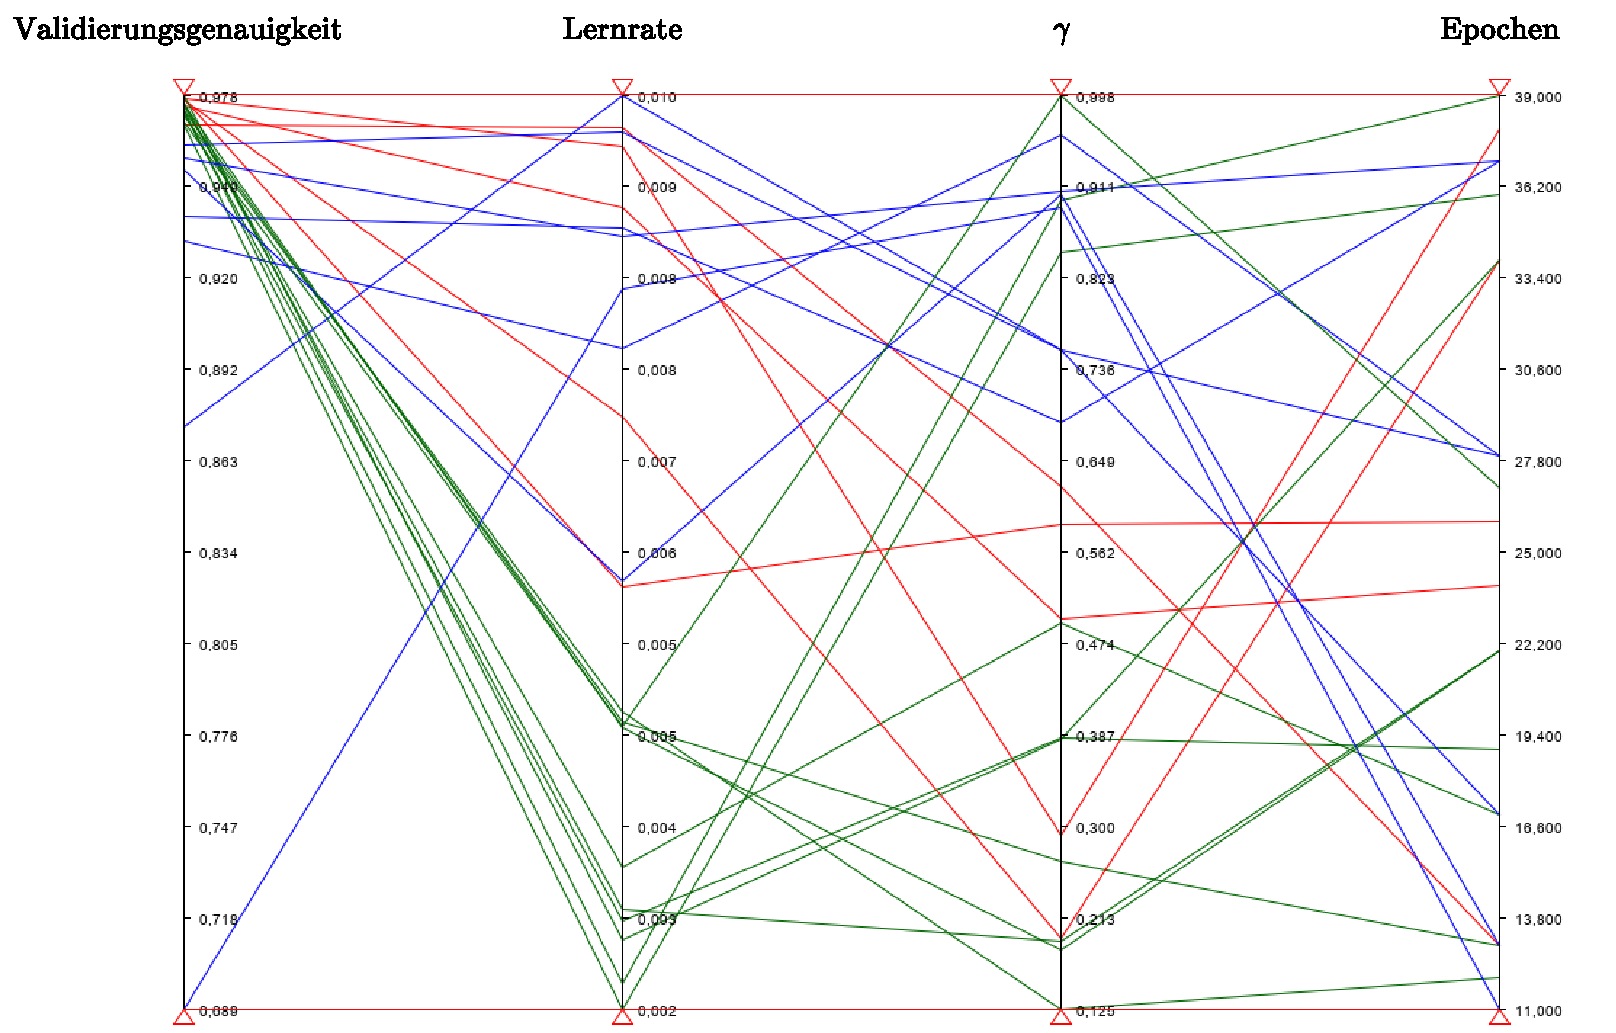
\includegraphics[scale=0.6]{NNOPT/finetuning_lr_gamma.pdf}
\caption{Einfluss von Lernrate und $\gamma$. Grün: Konfigurationen mit niedriger Lernrate $(<0.005)$, Rot: Hohe Lernrate und niedriges $\gamma$ $(<0.65)$, Blau: Hohe Lernrate und hohes $\gamma$}
\label{finetuning_lr_gamma}
\end{figure}
\\
\begin{figure}[h]
\centering
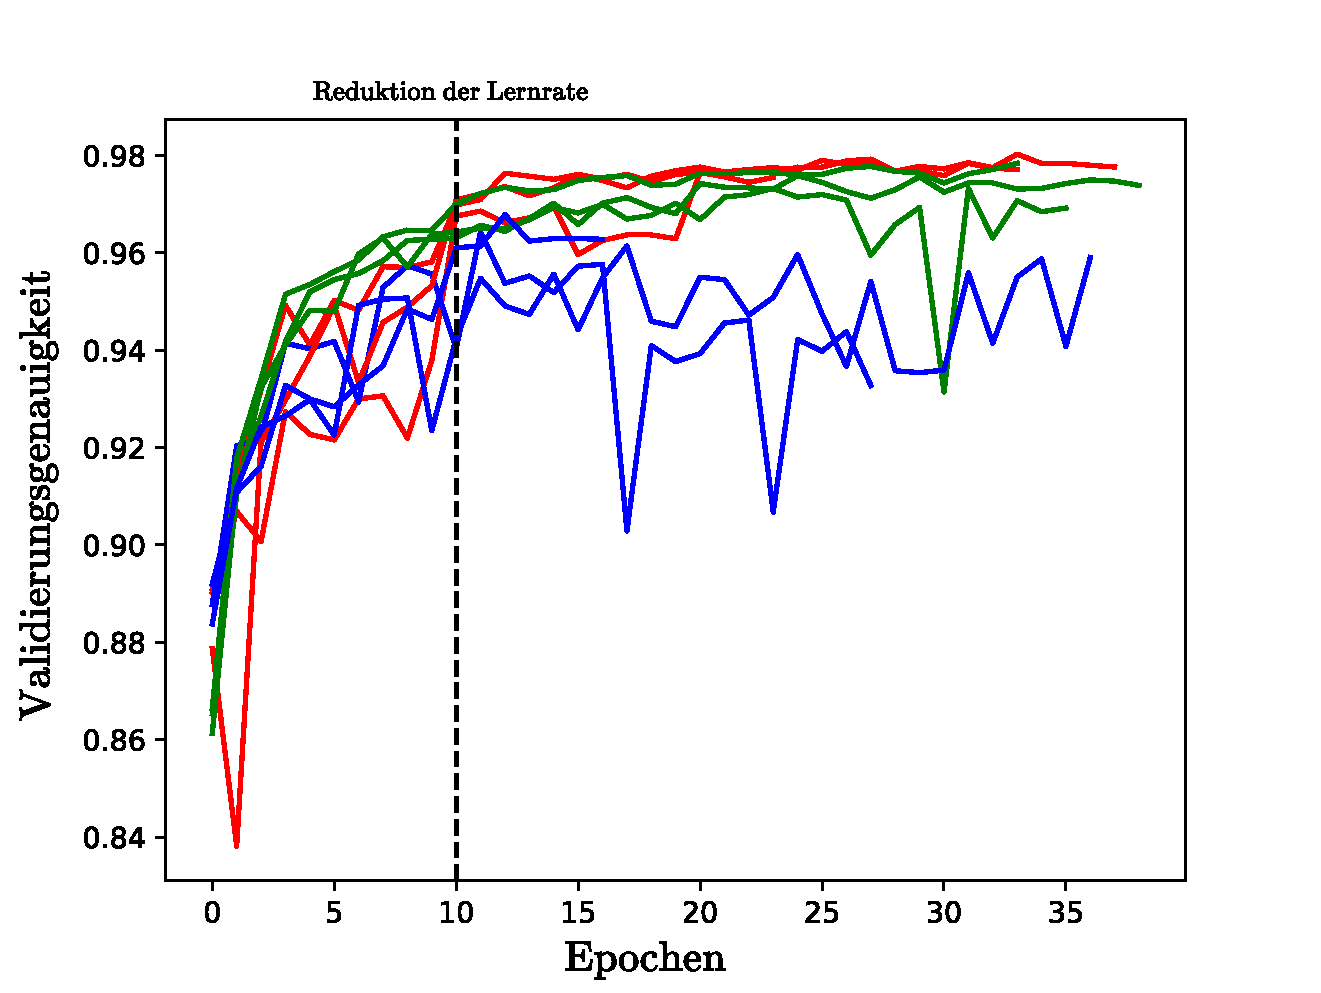
\includegraphics[scale=0.6]{NNOPT/finetuning_lr_gamma_verlauf.pdf}
\caption{Trainingsverlauf der Finetunings, bei unterschiedlicher Lernrate und $\gamma$. Farbgebung analog zu Abb.\ref{finetuning_lr_gamma}}
\label{finetuning_lr_gamma_verlauf}
\end{figure}
%zusammenhang zu lr und gamma
%optimale werte
%wie weiter trainiert wurde




%Ergebnisse
%Generell kann das Resnet die gestellten Aufgaben gut lösen. Das ganze funktioniert mit unterschiedlichen parametern noch sehr gut, daher legen wir keinen sehr großen fokus auf die hyperparamter.
%Finetuning funktioniert gut. Im Finetuningteil ist die Performance schon ob der ersten epoche sehr gut, was nahelegt, dass die netzwerkparameter nur noch wenig angepasst werden (müssen).
% Im Attention training ist schwieriger, da ein teil neuinitialisiert wird. Das obwohl die anzahl der optimierbaren parameter deutlich geringer ist.
% Da bei den meisten runs bereits sehr gute ergebnisse erzielt wurden und nicht mehr viel potential zur verbesserung besteht wurden nicht noch mehr experimente durchgeführt. In Anbetracht der Anzahl an Trails gegenüber den mögliche Suchraums lassen sich keine eindeutlgen/belastbaren Beziehungen gegenüber den hyperparametern festlegen. Es zeigen sich jedoch einige Tendenzen.
% mehr Epochen hat mehr potential
% Lernrate gibt es für attentiontraining einen sweetspot auch sonst tendenzen. 
% Beim Finetuning auch eher niedrige besser oder mit hohem gamma, damit die lernrate sich später einkriegt
% Ist die Lernrate sehr/zu hoch ist das trainingsverhalten insgesamt instabiler. Dazu mehrer lineplots vereinen
 